% BODHI MULE HUNTER AI - CyberShield Hackathon 2026 Prototype Report
% Built with the supplied CyberShield template (spconf.sty + IEEEbib.bst).
%
% Every number in this paper is a macro defined in results.tex, which is
% generated directly from artifacts/metrics/evaluation.json by
% scripts/render_report_numbers.py. Nothing quantitative is typed by hand, so
% the paper and the measured results cannot drift apart.
%
% Build:  make -C docs/report        (or: pdflatex; bibtex; pdflatex; pdflatex)

\documentclass{article}
\usepackage{spconf,amsmath,graphicx,hyperref,booktabs,url}

% Rupee sign without depending on a font package that may not be installed.
\providecommand{\rupee}{\textsf{Rs.}\,}

% ---------------------------------------------------------------
% AUTO-GENERATED by scripts/render_report_numbers.py - do not edit.
% Source: artifacts/metrics/evaluation.json
% Generated: 2026-07-28T17:19:51.671671+00:00
% ---------------------------------------------------------------

% --- dataset ---
\newcommand{\dsAccounts}{12{,}000}
\newcommand{\dsTransactions}{834{,}738}
\newcommand{\dsMules}{151}
\newcommand{\dsMuleRate}{1.26\%}
\newcommand{\dsRings}{21}
\newcommand{\dsDays}{120}
\newcommand{\dsFraudTxn}{2{,}121}
\newcommand{\dsTickets}{281}

% --- per-layer performance ---
\newcommand{\aucXgb}{0.9946}
\newcommand{\apXgb}{0.9540}
\newcommand{\precOneXgb}{0.983}
\newcommand{\recOneXgb}{0.781}
\newcommand{\aucSage}{0.9962}
\newcommand{\apSage}{0.9481}
\newcommand{\precOneSage}{0.983}
\newcommand{\recOneSage}{0.781}
\newcommand{\aucTgn}{0.9628}
\newcommand{\apTgn}{0.8036}
\newcommand{\precOneTgn}{0.892}
\newcommand{\recOneTgn}{0.709}
\newcommand{\aucIntel}{0.6883}
\newcommand{\apIntel}{0.3774}
\newcommand{\precOneIntel}{0.475}
\newcommand{\recOneIntel}{0.378}
\newcommand{\aucFused}{0.9966}
\newcommand{\apFused}{0.9707}
\newcommand{\precOneFused}{0.992}
\newcommand{\recOneFused}{0.788}

% --- calibration ---
\newcommand{\brier}{0.00125}
\newcommand{\ece}{0.0047}

% --- rule-engine baseline ---
\newcommand{\ruleAlerts}{9{,}647}
\newcommand{\ruleTP}{128}
\newcommand{\ruleFP}{9{,}519}
\newcommand{\rulePrecision}{1.33\%}
\newcommand{\ruleRecall}{84.8\%}
\newcommand{\bodhiAlerts}{129}
\newcommand{\bodhiTP}{128}
\newcommand{\bodhiFP}{1}
\newcommand{\bodhiPrecision}{99.22\%}
\newcommand{\fpReduction}{99.99\%}
\newcommand{\precUplift}{75$\times$}

% --- latency ---
\newcommand{\latPfifty}{0.054}
\newcommand{\latPninetynine}{0.113}
\newcommand{\throughput}{16{,}677}

% --- independence from the government feed ---
\newcommand{\indepShare}{64\%}
\newcommand{\indepDetected}{94}
\newcommand{\indepRecall}{95.9\%}

% --- out-of-time ---
\newcommand{\ootRings}{3}
\newcommand{\ootMules}{26}
\newcommand{\ootRecall}{100.0\%}

% --- detection lead time ---
\newcommand{\leadMedian}{11.5}
\newcommand{\leadSpacing}{92}
\newcommand{\leadEligible}{11}
\newcommand{\leadBeforeShare}{55\%}
\newcommand{\leadNeverTicketed}{16}
\newcommand{\weakNameA}{Smurfing}
\newcommand{\weakRecallA}{88.9\%}
\newcommand{\weakNameB}{Fan In Aggregation}
\newcommand{\weakRecallB}{93.3\%}
\newcommand{\weakNameC}{Layering Chain}
\newcommand{\weakRecallC}{98.3\%}
\newcommand{\decoyLegitimateDormantWakeN}{168}
\newcommand{\decoyLegitimateDormantWakeFP}{3.57\%}
\newcommand{\decoyCommunityCollectorN}{107}
\newcommand{\decoyCommunityCollectorFP}{2.80\%}
\newcommand{\decoyOrdinaryRetailN}{10{,}504}
\newcommand{\decoyOrdinaryRetailFP}{0.77\%}
\newcommand{\decoyBcAgentDeviceClusterN}{302}
\newcommand{\decoyBcAgentDeviceClusterFP}{0.33\%}
\newcommand{\decoySmallBusinessFanInN}{168}
\newcommand{\decoySmallBusinessFanInFP}{0.00\%}
\newcommand{\decoyMerchantN}{600}
\newcommand{\decoyMerchantFP}{0.00\%}

% --- organisers' alert dataset (bodhi/boi) ---
\newcommand{\boiColumns}{3{,}924}
\newcommand{\boiRows}{3{,}200}
\newcommand{\boiPositives}{186}
\newcommand{\boiStrategy}{\texttt{bank\_finalized}}
\newcommand{\boiHoldoutAuc}{0.7046}
\newcommand{\boiCvAuc}{0.7116}
\newcommand{\boiPrClean}{0.177}
\newcommand{\boiPrLeaked}{0.972}
\newcommand{\boiLeakMultiple}{5.5}
\newcommand{\boiBankN}{18}
\newcommand{\boiBankAuc}{0.712}
\newcommand{\boiBankPr}{0.177}
\newcommand{\boiBankEngN}{2{,}028}
\newcommand{\boiBankEngAuc}{0.651}
\newcommand{\boiBankEngPr}{0.163}
\newcommand{\boiTopKN}{131}
\newcommand{\boiTopKAuc}{0.622}
\newcommand{\boiTopKPr}{0.137}
\newcommand{\boiAllN}{5{,}926}
\newcommand{\boiAllAuc}{0.618}
\newcommand{\boiAllPr}{0.112}


\title{BODHI MULE HUNTER AI: Explainable Graph-Temporal Detection of\\
       Money-Mule Accounts and Suspicious Transactions}

\name{Akshay Tiwari$^{1}$ \quad Palak Vishwakarma$^{2}$ \quad
      Archi Singh Rajput$^{3}$ \quad Kartik Jain$^{4}$%
\thanks{Enrolment numbers: $^{1}$0246CS241037, $^{2}$0246AL241124,
$^{3}$0246CS240174, $^{4}$0246AL241094. Prototype submission for the
CyberShield Hackathon 2026, Problem Statement~2, in association with Bank of
India and IIT Hyderabad. Source, data simulator and reproduction scripts are
released with this report.}}
\address{Team BODHI --- CyberShield Hackathon 2026, Problem Statement 2}

\begin{document}
\maketitle

\begin{abstract}
Money mules convert stolen funds into untraceable cash, and rule-based
transaction monitoring detects them at a precision so low that analysts cannot
act on the output. We present BODHI MULE HUNTER AI, a nine-layer engine that
fuses gradient-boosted tabular screening, an inductive graph neural network and
a temporal memory network over each account's event sequence, calibrated into a
single supervisory risk score. On a simulated bank of \dsAccounts{} accounts and
\dsTransactions{} cross-channel transactions containing seven documented
laundering typologies, the fused model reaches \aucFused{} ROC-AUC and
\apFused{} PR-AUC. Against a rule engine of the kind banks deploy today, at
identical recall, alert volume falls from \ruleAlerts{} to \bodhiAlerts{} and
precision rises from \rulePrecision{} to \bodhiPrecision{} --- \fpReduction{} of
false positives eliminated. Inline decisions complete in \latPfifty{}\,ms at the
median. Every alert carries exact Shapley attributions and a learned
edge-importance mask, and the containment layer refuses to act autonomously
without corroboration from independent model layers.
\end{abstract}

\begin{keywords}
money mule detection, graph neural networks, temporal graph networks,
explainable AI, anti-money laundering
\end{keywords}

% =====================================================================
\section{Introduction}
\label{sec:intro}

A money mule is an account whose owner has rented, sold, or been deceived into
lending it. Criminal proceeds are pushed into it, split, relayed through several
further accounts, and withdrawn as cash --- typically within hours. The account
itself is unremarkable: the KYC is genuine, the customer exists, the payments
clear. What is anomalous is the \emph{shape} of the money passing through it and
the \emph{company it keeps}.

This creates a specific failure mode for the transaction-monitoring systems
banks currently operate. Threshold-and-scenario engines evaluate accounts in
isolation, so they cannot express "this account's counterparties are themselves
suspicious" or "these forty credits arrived in ninety minutes and left at
03:12". Lacking that vocabulary, they compensate with sensitivity, and the
result is an alert queue an AML desk cannot clear. The baseline we implement in
Section~\ref{sec:results} raises \ruleAlerts{} alerts at \rulePrecision{}
precision: ninety-nine of every hundred investigations are wasted.

We make four contributions.

\begin{enumerate}
\item \textbf{A three-view ensemble.} Rather than three variants of the same
tabular model, we combine a gradient-boosted model over behavioural aggregates,
a GraphSAGE network over an account--device--IP graph, and a temporal graph
network over each account's ordered event stream. Section~\ref{sec:models}
shows that these views are genuinely complementary.

\item \textbf{Explainability that survives contact with a regulator.} Layer~4
uses exact TreeSHAP, whose attributions sum to the model's margin rather than
approximating it; Layer~5 uses a GNNExplainer edge mask, which answers the
question SHAP structurally cannot --- \emph{which relationships} drove the
score. Both are rendered into the vocabulary of an AML officer and populate the
grounds-of-suspicion section of a draft Suspicious Transaction Report.

\item \textbf{An evaluation designed to be falsifiable.} Synthetic fraud data
makes any model look excellent. We therefore plant legitimate populations that
are structurally indistinguishable from mules --- Business Correspondent agents
operating many accounts from one handheld, chit-fund collectors with burst
fan-in, near-threshold property payments --- and report the false-positive rate
on each one separately.

\item \textbf{Containment that can refuse.} The automated kill-switch requires
corroboration from at least two independent model layers before it may freeze an
account, is rate-limited, time-limited, reversible, and excludes salary and
pension accounts entirely. Every refusal is audited.
\end{enumerate}

% =====================================================================
\section{Problem setting and data}
\label{sec:data}

\subsection{Why a simulator}

Account-level mule labels joined to device, IP and UPI linkage are
simultaneously commercially sensitive, personally identifying and legally
restricted; no bank can export them and no public dataset contains them. The
alternative to simulation is not real data --- it is no evaluation at all.

We therefore built a generator that reproduces the structures the detector must
find. It produces \dsAccounts{} accounts over \dsDays{} days,
\dsTransactions{} transactions across eight payment rails (UPI, IMPS, NEFT,
RTGS, AePS, ATM, card, wallet), \dsMules{} mule accounts (\dsMuleRate{}) in
\dsRings{} rings, and \dsTickets{} government cyber-fraud tickets arriving with
realistic reporting lag.

\subsection{Typologies}

Seven laundering patterns from FIU-IND and FATF guidance are implemented
literally, so that recall can be reported \emph{per typology} rather than as an
average that hides blind spots: fan-in aggregation, multi-hop layering chains,
structuring (smurfing), dormant reactivation bursts, device-farm account rental,
rapid cash-out, and malicious-APK harvest networks.

\subsection{The hard negatives}

This is the part of the data design that determines whether any precision figure
means anything. A collection mule receiving forty payments from strangers in one
afternoon is structurally identical to a tuition-batch organiser. We plant, as
\emph{legitimate} accounts:

\begin{itemize}
\item \textbf{Business Correspondent (Bank Mitra) agents} ---
\decoyBcAgentDeviceClusterN{} accounts where one handheld device legitimately
serves many customers and dispenses AePS cash all day. This is the exact
fingerprint of a device farm performing rapid cash-out.
\item \textbf{Community collectors} --- \decoyCommunityCollectorN{} chit-fund and
festival-committee organisers with burst fan-in from strangers, forwarding
$\sim$90\% of receipts within hours.
\item \textbf{Small businesses} --- \decoySmallBusinessFanInN{} accounts with
heavy daily peer-to-peer fan-in from unrelated payers.
\item \textbf{Genuine dormancy breaks} --- \decoyLegitimateDormantWakeN{} student
and non-resident accounts waking after months of silence.
\item \textbf{Near-threshold payers} --- repeated legitimate transfers parked
just under the channel limit for property and jewellery purchases.
\end{itemize}

Without these populations the models score above $0.999$ AUC and the exercise is
meaningless.

% =====================================================================
\section{System architecture}
\label{sec:arch}

The engine is organised as nine layers, each owned by a named agent with a
declared input and output contract so that the provenance of every decision is
recoverable from the audit trail.

\noindent\textbf{Layer 1 --- Ingestion.} Normalises cross-channel transactions,
government cyber-fraud tickets (NCRP/I4C/1930), APK-derived indicators, and
regulatory directives. The four directive classes are handled distinctly: a mule
list raises a score floor; a velocity limit changes a decision \emph{threshold},
not a score; a sanction is absolute; an advisory is recorded and surfaced but
never auto-applied, because a machine cannot responsibly convert prose into an
enforcement rule.

\noindent\textbf{Layer 2 --- Feature engineering.} Sixty behavioural features:
velocity, fan-in/fan-out ratios, dormancy, burst scores, structuring share,
device reuse, pass-through ratios and channel mix. Every builder is
point-in-time correct --- nothing after the evaluation instant is visible --- and
a regression test asserts that passing an \texttt{as\_of} argument is identical
to truncating the ledger by hand. A second test shuffles the labels and asserts
the feature matrix is unchanged, which forecloses label leakage.

\noindent\textbf{Layer 3 --- Graph construction.} Accounts are nodes; edges are
money transfers, shared devices and shared IP addresses. Shared-identifier
cliques are capped: an identifier behind more than twenty-five accounts is
infrastructure --- a CGNAT pool, a banking kiosk --- not evidence of collusion.
Without the cap a single public address produces a four-thousand-node clique and
the graph layer becomes a false-positive generator.

\noindent\textbf{Layers 4--6 --- Three views.} Described in
Section~\ref{sec:models}.

\noindent\textbf{Layer 7 --- Fusion.} Section~\ref{sec:fusion}.

\noindent\textbf{Layer 8 --- Explainability.} TreeSHAP, GNNExplainer, and a
narrative generator that maps each feature onto a sentence in the vocabulary of
an AML desk.

\noindent\textbf{Layer 9 --- Alerting and containment.}
Section~\ref{sec:containment}.

% =====================================================================
\section{The three model views}
\label{sec:models}

The central design claim is that mule detection needs three genuinely different
kinds of evidence, and that no single model family supplies all three.

\subsection{Layer 4: gradient-boosted screening}

An XGBoost classifier over the sixty behavioural features disposes of the
overwhelming majority of accounts cheaply. It was chosen over a neural tabular
model for one reason: exact TreeSHAP. Shapley values for tree ensembles are
computable in polynomial time, so the attribution shown to an investigator is
not a sampled approximation --- it sums to the model's raw margin, a property we
assert in the test suite, and it is stable across runs. That matters when the
explanation is transcribed into a regulatory filing.

The class-imbalance weight is capped rather than set to the full negative-to-
positive ratio. Uncapped, on a \dsMuleRate{} base rate, it destroys calibration,
and a mis-calibrated score cannot be allowed to drive an automated freeze.

\subsection{Layer 5: inductive graph learning}

We use the mean-aggregator GraphSAGE formulation \cite{hamilton2017}:
%
\begin{equation}
h_v^{(k)} = \mathrm{ReLU}\!\left(
  W_{\text{self}}^{(k)} h_v^{(k-1)} +
  W_{\text{neigh}}^{(k)} \!\!\!\underset{u \in \mathcal{N}(v)}{\mathrm{MEAN}}\!\!\! h_u^{(k-1)}
\right)
\end{equation}
%
with two layers and a deterministic top-$k$ fan-out cap standing in for random
neighbour sampling. Determinism is a requirement, not a simplification: an
investigator re-opening a case tomorrow must see the same score. Because the
weights never index a node identity, the model is genuinely inductive --- an
account opened this morning is scored from its neighbourhood alone.

\subsection{Layer 6: temporal memory}

The memory module of a Temporal Graph Network \cite{rossi2020} is a gated
recurrent unit updated on every interaction, with elapsed time injected through
a learnable encoding. We implement exactly that over each account's most recent
sixty-four events.

This layer exists because aggregates destroy the signal that matters most.
``Received \rupee4 lakh from 38 payers over the month'' describes a shopkeeper
and a mule equally well. ``Received \rupee4 lakh from 38 payers between 14:10 and
15:40, then withdrew \rupee3.8 lakh in nineteen ATM visits beginning at 03:12''
describes only one of them. Order is the discriminant, and no aggregate
preserves it.

\subsection{Implementation note}

Both neural layers are implemented in NumPy with analytically derived gradients
rather than in a deep-learning framework. The motivation is deployability in a
bank: the entire engine installs from four wheels, runs on a laptop CPU, and
presents no GPU or CUDA surface to certify. Because ``hand-derived'' is a
plausible source of silent error, every parameter tensor's analytic gradient is
verified against central finite differences in the test suite.

% =====================================================================
\section{Fusion and calibration}
\label{sec:fusion}

The four channel scores --- tabular, graph, temporal and external intelligence
--- are blended in log-odds space. Sub-scores accumulate against $0$ and $1$,
where a linear model in probability space cannot separate $0.990$ from $0.9999$;
that is a hundredfold difference in odds and precisely the region in which alert
ranking is decided.

Two properties are enforced rather than hoped for.

\noindent\textbf{Monotonicity.} Blend weights are constrained non-negative, so
the fused score can never decrease when a layer's evidence increases. This is
not a regularisation convenience. An unconstrained stacker fitted on a small
fold reliably learns a negative coefficient on the temporal channel, which is
indefensible in front of an investigator and unshippable past a supervisor. A
useful side effect is that the blend can always degenerate to ``all weight on
the single best layer'', so fusion cannot perform much worse than its best
input.

\noindent\textbf{Calibration.} Isotonic regression maps the blend onto observed
frequencies, giving a Brier score of \brier{} and expected calibration error of
\ece{}. Isotonic regression is a step function, so on a near-separable problem
it collapses thousands of distinct scores into a handful of plateaus and every
account within a plateau becomes tied; we measured a four-point AUC loss from
those ties. Retaining a two-percent share of the underlying monotone score
breaks them without disturbing calibration.

The blend is fitted on a fourth, dedicated fold. A stacker fitted on the
validation fold --- the fold that early-stopped its own inputs --- inherits their
optimism and, in our experiments, performed \emph{worse} than the best single
layer.

% =====================================================================
\section{Results}
\label{sec:results}

\subsection{Detection performance}

Table~\ref{tab:layers} reports each layer on the held-out data. The
complementarity claim of Section~\ref{sec:models} is visible: the fused model
exceeds every individual view on both ranking metrics.

\begin{table}[htb]
\centering
\caption{Per-layer detection performance. P@1\% and R@1\% are precision and
recall within an alert budget of one percent of accounts --- the quantity an
analyst actually experiences.}
\label{tab:layers}
\begin{tabular}{lrrrr}
\toprule
Layer & ROC-AUC & PR-AUC & P@1\% & R@1\% \\
\midrule
L4 XGBoost   & \aucXgb   & \apXgb   & \precOneXgb   & \recOneXgb \\
L5 GraphSAGE & \aucSage  & \apSage  & \precOneSage  & \recOneSage \\
L6 TGN       & \aucTgn   & \apTgn   & \precOneTgn   & \recOneTgn \\
Intelligence & \aucIntel & \apIntel & \precOneIntel & \recOneIntel \\
\midrule
\textbf{L7 Fused} & \textbf{\aucFused} & \textbf{\apFused} &
\textbf{\precOneFused} & \textbf{\recOneFused} \\
\bottomrule
\end{tabular}
\end{table}

\subsection{Against the incumbent}

We implement a rule engine of the kind banks deploy today --- eight scenarios
covering velocity, structuring, dormancy, cash-out ratio, device sharing,
new-account turnover and off-hours concentration --- and give it its best
operating point rather than a strawman. The comparison is made at
\emph{identical recall}, because a system that alerts on everything can always
claim to catch more.

\begin{table}[htb]
\centering
\caption{Rule engine versus BODHI at equal recall (\ruleRecall).}
\label{tab:baseline}
\begin{tabular}{lrr}
\toprule
 & Rule engine & BODHI \\
\midrule
Alerts raised    & \ruleAlerts    & \textbf{\bodhiAlerts} \\
True positives   & \ruleTP        & \bodhiTP \\
False positives  & \ruleFP        & \textbf{\bodhiFP} \\
Precision        & \rulePrecision & \textbf{\bodhiPrecision} \\
\bottomrule
\end{tabular}
\end{table}

\fpReduction{} of false positives are eliminated at unchanged recall, a
\precUplift{} precision uplift. In operational terms an analyst clears the same
true positives while opening \bodhiAlerts{} cases instead of \ruleAlerts{}.

\subsection{Robustness checks}

\noindent\textbf{Behaviour on the planted decoys.} At the alert threshold, the
false-positive rate is \decoyBcAgentDeviceClusterFP{} on Business Correspondent
device clusters, \decoyCommunityCollectorFP{} on community collectors,
\decoySmallBusinessFanInFP{} on small businesses with heavy fan-in, and
\decoyOrdinaryRetailFP{} on ordinary retail accounts. These are the numbers that
make Table~\ref{tab:baseline} credible.

\noindent\textbf{Out-of-time generalisation.} \ootRings{} rings activate only in
the final quarter of the simulation window and are therefore genuinely unseen
patterns. Recall on their \ootMules{} member accounts is \ootRecall{}.

\noindent\textbf{Independence from the government feed.} The supervised layers
never receive ticket data --- the intelligence features are a disjoint set,
asserted by test, and enter only at Layer~7. Consequently \indepShare{} of
detected mules were never named in any NCRP ticket: they are cases the
government feed could not have supplied.

\noindent\textbf{Latency.} Inline decisions complete in \latPfifty{}\,ms at the
median and \latPninetynine{}\,ms at the 99th percentile, roughly
\throughput{} decisions per second per core. This is achievable because the
graph and temporal layers run on a schedule and cache a standing risk per
account; the authorisation path combines those cached scores with the
transaction's own attributes and never traverses the graph.

\subsection{Where the system is weak}

Recall is not uniform, and averaging conceals that. The weakest typology is
\weakNameA{} at \weakRecallA{} recall, followed by \weakNameB{} at
\weakRecallB{}. The structuring result is expected and structural: an individual
sub-threshold transfer is, by construction, indistinguishable from a genuine
near-threshold payment, so detection depends on an aggregate pattern that only
becomes visible once enough transfers have accumulated. Terminal cash-out
accounts are similarly hard because they have short, thin histories --- they
receive once and drain.

We report these rather than averaging them away, because a deployment team needs
to know which typologies still require human-designed scenarios alongside the
model.

\begin{figure}[htb]
\begin{minipage}[b]{1.0\linewidth}
  \centering
  \centerline{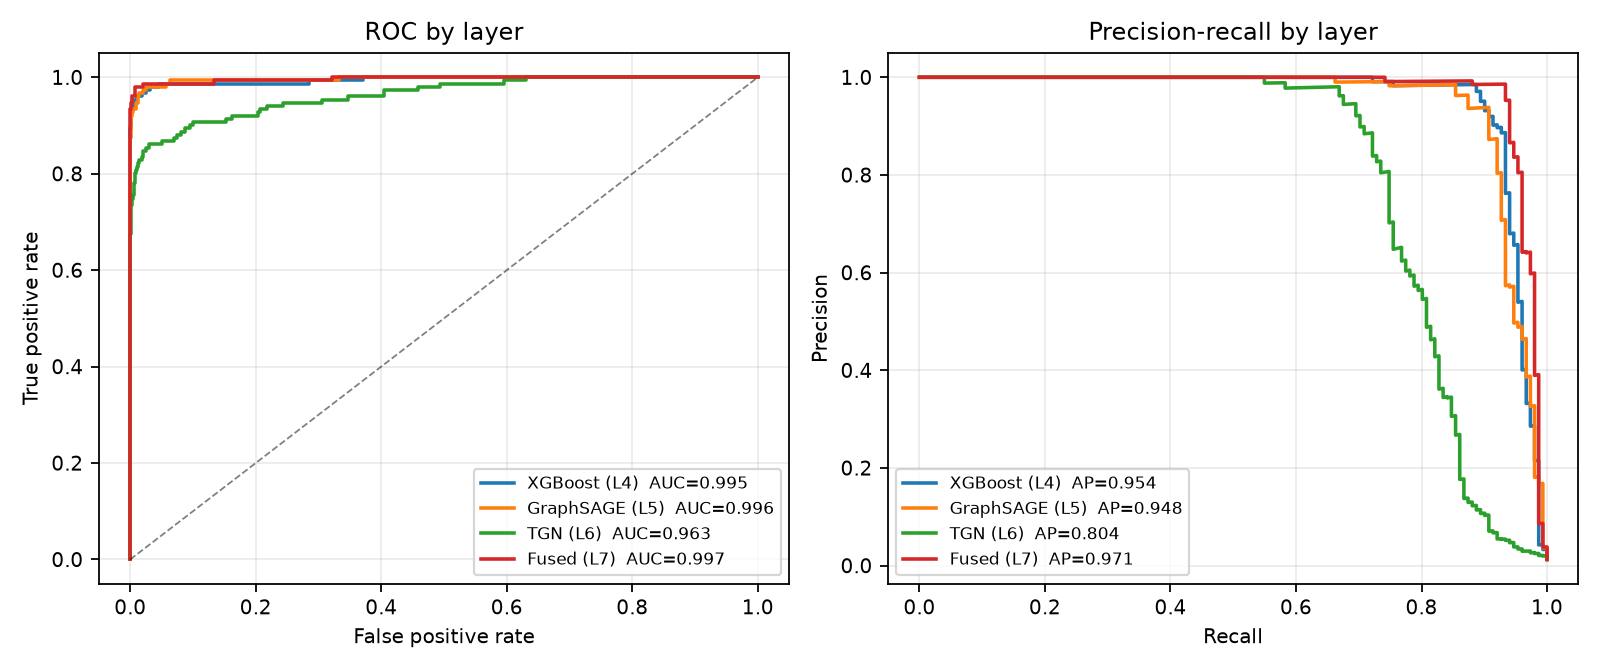
\includegraphics[width=8.5cm]{figures/roc_pr}}
  \centerline{(a) ROC and precision--recall by layer}\medskip
\end{minipage}
\begin{minipage}[b]{.48\linewidth}
  \centering
  \centerline{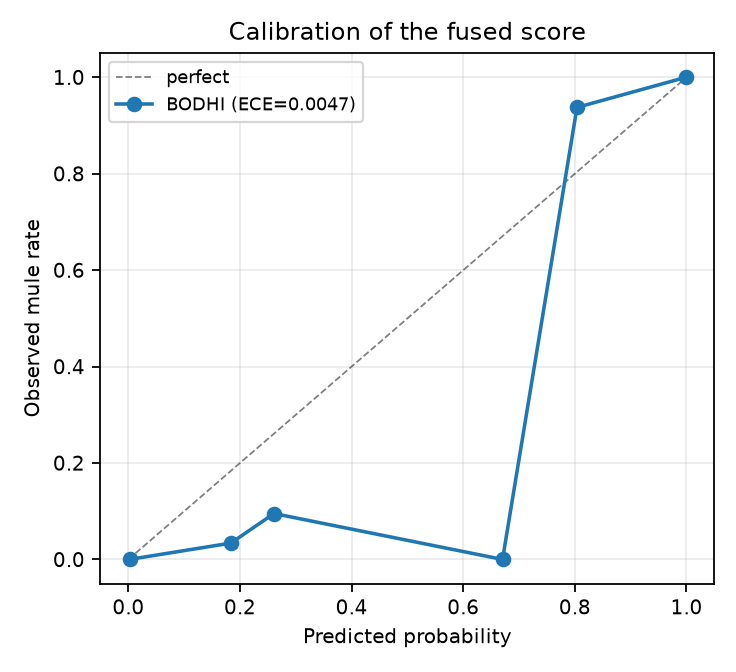
\includegraphics[width=4.0cm]{figures/calibration}}
  \centerline{(b) Calibration}\medskip
\end{minipage}
\hfill
\begin{minipage}[b]{0.48\linewidth}
  \centering
  \centerline{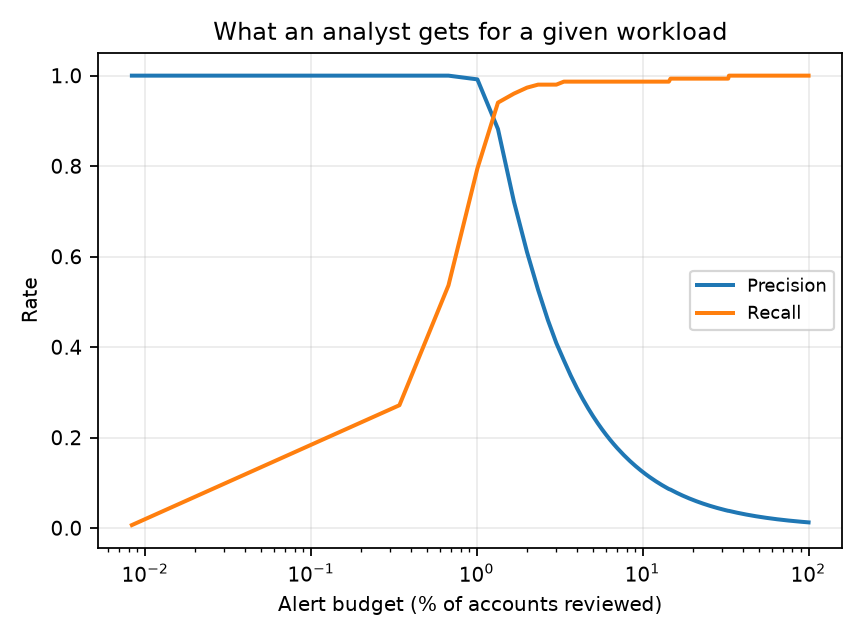
\includegraphics[width=4.0cm]{figures/alert_budget}}
  \centerline{(c) Precision and recall versus analyst workload}\medskip
\end{minipage}
\caption{Evaluation summary. All panels are regenerated by
\texttt{make evaluate}.}
\label{fig:res}
\end{figure}

% =====================================================================
\section{Explainability}
\label{sec:explain}

An alert reading \texttt{rapid\_passthrough\_ratio = 0.94, SHAP +1.31} is
unusable by the officer who must telephone the customer. The narrative layer
maps every feature onto a sentence in the vocabulary of the desk: \emph{``94\% of
every rupee credited left the account within sixty minutes --- the account is a
conduit, not a destination.''} The mapping is held as data rather than code, so
the wording that eventually reaches a supervisor remains reviewable in one
place, and a test asserts that no raw feature identifier leaks into
investigator-facing text.

Structural evidence is handled separately. GNNExplainer \cite{ying2019} learns a
soft mask over the edges of the target account's two-hop neighbourhood,
optimised so that the masked sub-graph reproduces the original prediction while
remaining sparse. This answers the question SHAP cannot express at all ---
\emph{which relationships} produced the score --- and for mule detection the
relationships are usually the entire case.

% =====================================================================
\section{Containment, safety and compliance}
\label{sec:containment}

Freezing an account is the most consequential action the system can take. A
wrongly frozen account is a person unable to pay for medicine, and no
improvement in AUC justifies treating that casually. The kill-switch is
therefore built from constraints rather than a threshold:

\begin{itemize}
\item \textbf{Proportionality.} Below the critical band the automation cannot
freeze at all; it may only hold an inbound credit or force step-up
authentication.
\item \textbf{Corroboration.} A full freeze requires at least two
\emph{independent} layers to agree, so a single layer's failure mode cannot
freeze anyone.
\item \textbf{Reversibility.} Every action carries a time-to-live and can be
reverted; reversal is itself an audited event.
\item \textbf{Rate limiting.} Automated freezes per hour are bounded, capping
the blast radius if a model degrades or an upstream feed is poisoned.
\item \textbf{Protected accounts.} Salary, pension and benefit accounts are
excluded from automated freezing entirely.
\end{itemize}

When a constraint fires, the action is \emph{downgraded} rather than escalated
and flagged for human review. Every decision, including every refusal, is
written to a hash-chained append-only audit log whose head hash is exposed for
external anchoring.

The compliance layer drafts Suspicious Transaction Reports populated from
exactly the evidence displayed to the investigator, so what the model asserted
and what the institution files cannot diverge. Drafts are explicitly marked as
requiring human sign-off; nothing is filed autonomously. Cash-transaction
reporting aggregates per account per calendar day, which is the level at which
the obligation applies --- and precisely why structuring defeats a
per-transaction check.

% =====================================================================
\section{Ecosystem synergy: BODHI SHIELD}
\label{sec:shield}

Mule networks are frequently seeded by malicious Android packages that carry
their beneficiary accounts hardcoded inside them. Our companion component
performs static triage of a submitted APK: it parses the binary
\texttt{AndroidManifest.xml} string pool to specification, scores permission
\emph{combinations} rather than individual permissions (READ\_SMS alone is a
messaging application; READ\_SMS together with an accessibility service and a
screen overlay is a banking trojan), mines the DEX for UPI handles, IFSC codes,
account numbers and command-and-control endpoints, and detects commercial
packers and identifier obfuscation.

Every financial identifier recovered is streamed into the Mule Hunter graph as a
weighted node. The consequence is architectural rather than incremental: when a
new trojan is analysed on the day it appears, the beneficiary accounts it was
built to pay already carry an elevated intelligence score before the first
victim installs it. Detection stops being purely retrospective.

% =====================================================================
\section{The organisers' alert dataset}
\label{sec:boi}

The organisers released the column dictionary for the Phase~2 dataset and stated
that the model would be scored on a validation file they had not shared. That
dataset is a different object from the one above: one row is a
transaction-monitoring \emph{alert}, not an account, so the population is already
pre-filtered by the bank's own rules and the task is triage rather than detection
from scratch. We therefore built a second pipeline (\texttt{bodhi/boi/}) directly
against the published schema of \boiColumns{} columns. Almost every predictor is
machine-generated from a compact grammar --- aggregation, customer- or
bank-induced, channel, direction, measure, observation window --- so the schema
module \emph{parses} the names rather than treating them as opaque. That is what
allows several thousand columns to be grouped into families measured across the
7-, 14- and 31-day windows, and what prevents \texttt{NON\_CASH\_CHQ} being
silently matched as \texttt{CASH}.

\subsection{Four columns leak the label}

The dictionary describes \texttt{FRAUD\_SUSPECTED}, \texttt{FALSE\_POSITIVE},
\texttt{OTHER\_RESOLUTION} and \texttt{UNATTENDED} as resolution-status flags:
they record how an analyst \emph{closed} the alert, and
\texttt{MIN\_RESOLVE\_DAYS} and \texttt{MAX\_RESOLVE\_DAYS} record how long that
took. An open alert --- the only kind worth scoring --- carries none of them.
Admitting them raises cross-validated PR-AUC from \boiPrClean{} to
\boiPrLeaked{}, a \boiLeakMultiple{}$\times$ jump, with \texttt{FRAUD\_SUSPECTED}
alone worth roughly a third of the gain and the six columns occupying the top
importance ranks. That is not a model; it is a lookup of the answer stored in a
different column. They are quarantined by default, and the flag that admits them
prints a warning while it does so.

\subsection{The bank's own eighteen features win}

The dictionary marks \boiBankN{} predictors as bank-finalised. The pipeline
treats that as a hypothesis rather than an instruction and competes four feature
strategies under repeated stratified cross-validation, with selection performed
\emph{inside} every fold (Table~\ref{tab:boi}).

\begin{table}[t]
\caption{Feature strategies, repeated stratified cross-validation}
\label{tab:boi}
\centering\small
\begin{tabular}{lrrr}
\hline
Strategy & Features & ROC-AUC & PR-AUC \\
\hline
Bank-finalised subset      & \boiBankN{}    & \boiBankAuc{}    & \boiBankPr{} \\
Bank subset $+$ engineered & \boiBankEngN{} & \boiBankEngAuc{} & \boiBankEngPr{} \\
Automatic top-$k$          & \boiTopKN{}    & \boiTopKAuc{}    & \boiTopKPr{} \\
Every available column     & \boiAllN{}     & \boiAllAuc{}     & \boiAllPr{} \\
\hline
\end{tabular}
\end{table}

The eighteen expert-chosen columns beat all \boiAllN{}, and beat automatic
selection. With \boiPositives{} positives against thousands of predictors this is
what statistical theory predicts, and it is precisely why the pipeline measures
instead of assuming. The untouched holdout scored \boiHoldoutAuc{} against a
cross-validated \boiCvAuc{} --- a gap small enough to be evidence that the
selection procedure is not inflating itself. A regression test makes the same
point adversarially: it shuffles the target, destroying all signal, and asserts
the reported AUC stays near chance, which a globally-selecting pipeline fails.

\emph{These numbers are not model performance.} The organisers' data had not been
released when this was built, so they were measured on a stand-in table generated
with their exact \boiColumns{}-column schema and a deliberately modest injected
signal. What they demonstrate is that the pipeline runs end to end, that the
methodology does not flatter itself, and that the leakage trap is real --- nothing
more. When the real file arrives, one command replaces every figure in this
section with a measured one.

% =====================================================================
\section{Limitations}
\label{sec:limits}

We state these plainly because a prototype that hides them is not useful to a
deployment team.

Results are on simulated data; they demonstrate that the architecture works and
that it decisively beats a rule engine on data containing realistic decoys, but
they are not a forecast of production performance. The SHIELD component performs
static analysis only --- the dynamic sandbox with runtime hooking described in
our proposal requires an instrumented Android image and cannot ship
self-contained. The graph layers are not real-time: a full re-score of the
population takes tens of seconds, so an account whose neighbourhood changed
since the last batch is scored on slightly stale structure. The system sees one
institution, so rings routing through several banks are only partly visible ---
a data-sharing problem rather than a modelling one. The strongest single feature
is neighbourhood risk propagated from confirmed cases, which means a cold start
with no known mules would perform materially worse. Finally, disparate impact is
unevaluated: minimum-KYC status and shared-device features are predictive but
correlate with lower-income and multi-occupancy households, and any real
deployment must measure alert-rate parity before go-live.

% =====================================================================
\section{Conclusion}
\label{sec:conclusion}

Mule detection fails today not because the signal is absent but because
single-account rule engines cannot express it. Giving the problem three
complementary views --- behavioural aggregates, network structure and event
ordering --- and fusing them under a monotonicity constraint into a calibrated
score reduces false positives by \fpReduction{} at unchanged recall relative to
a realistic incumbent, while producing explanations specific enough to file and
containment actions cautious enough to automate. The same discipline is applied
to the organisers' own alert schema, where the honest finding is that four of its
columns encode the answer and the bank's eighteen expert-chosen features beat
automatic selection over several thousand. The complete system, the data
simulator and every script needed to reproduce these numbers are released
alongside this report.

% =====================================================================
\vfill\pagebreak

\bibliographystyle{IEEEbib}
\bibliography{refs}

\end{document}
